\documentclass[tikz,border=5mm]{standalone}
\usepackage{amsmath, amssymb}
\usetikzlibrary{arrows.meta, decorations.markings}

% Define styles for arrows and annotations
\tikzset{
    myarrow/.style={-{Latex[scale=1.2]}},
    projarrow/.style={->, shorten >=1pt, shorten <=1pt},
    dot/.style={circle, fill, inner sep=1.5pt}
}

\begin{document}
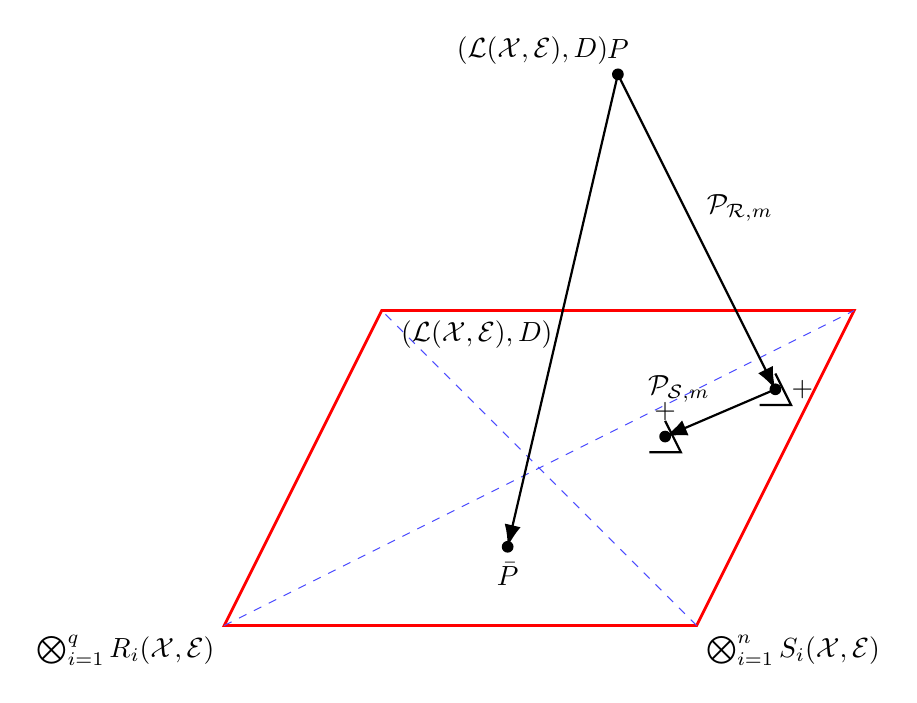
\begin{tikzpicture}[scale=2]

% Define coordinates for the parallelogram
\coordinate (A) at (0,0);
\coordinate (B) at (3,0);
\coordinate (C) at (4,2);
\coordinate (D) at (1,2);

% Draw the parallelogram
\draw[red, line width=1pt] (A) -- (B) -- (C) -- (D) -- cycle;

% Draw the interior diagonal lines
\draw[blue!70, dashed] (A) -- (C);
\draw[blue!70, dashed] (B) -- (D);

% Label the bottom edges
\node[below left] at (A) {$\bigotimes_{i=1}^{q} R_i(\mathcal{X},\mathcal{E})$};
\node[below right] at (B) {$\bigotimes_{i=1}^n S_i(\mathcal{X},\mathcal{E})$};

% Add points P, P_R, P_S, and P_bar
\coordinate (P) at (2.5, 3.5);
\coordinate (P_R) at (3.5, 1.5);
\coordinate (P_S) at (2.8, 1.2);
\coordinate (P_bar) at (1.8, 0.5);

% Draw the vectors and their projections
\draw[myarrow, thick] (P) -- (P_R) node[midway, above right] {$\mathcal{P}_{\mathcal{R},m}$};
\draw[myarrow, thick] (P_R) -- (P_S) node[midway, above left] {$\mathcal{P}_{\mathcal{S},m}$};
\draw[myarrow, thick] (P) -- (P_bar) node[midway, below left] {$(\mathcal{L}(\mathcal{X},\mathcal{E}), D)$};

% Mark the points with dots
\node[dot, label=above:$P$] at (P) {};
\node[dot, label=right:$+$] at (P_R) {};
\node[dot, label=above:$+$] at (P_S) {};
\node[dot, label=below:$\bar{P}$] at (P_bar) {};

% Add the label for the top-left point
\node[above left] at (P) {$(\mathcal{L}(\mathcal{X},\mathcal{E}), D)$};

% Add perpendicular marks
\draw[thick] (P_R) ++(-0.1,-0.1) -- ++(0.2,0) -- ++(-0.1,0.2);
\draw[thick] (P_S) ++(-0.1,-0.1) -- ++(0.2,0) -- ++(-0.1,0.2);

\end{tikzpicture}
\end{document}